% Appendix on FED phase and delay scans

This section will describe some aspects of determining the  so called 'phase' and 'delay' of the FED. The sample  plots shown in this section are taken from runs on the  FPIX pilot run detector. this was done using a version 4 FED with the Aug. 22, 2007 firmware version.

In order to get the transparent data to 'look' OK I had to send an LRES before each trigger. Will Johns and I had  long email exchanges trying to understand this. I think that the final conclusion was that the FED state machine gets confused when the input data is non standard. In the scans over phases and delays there are certain settings that are invalid, i.e., that you try to read out the ADC before the data is available. At the end of this section I will discuss two issues that I noticed in looking at the transparent data. 
For the above reason we also turn off the automatic baseline correction to avoid it getting confused if you seend non valid  data or if you don't have correct address levels.

In these tests we take 10 triggers for each delay and phase setting. I'll show plots, as in Fig.~\ref{fig:phasedelayraw}, where for each of the two possible phases the profile histogram shows the adc value as a function of clock+delay/16. The third plots just shows the two plots on top of each other.

\begin{figure}
\begin{center}
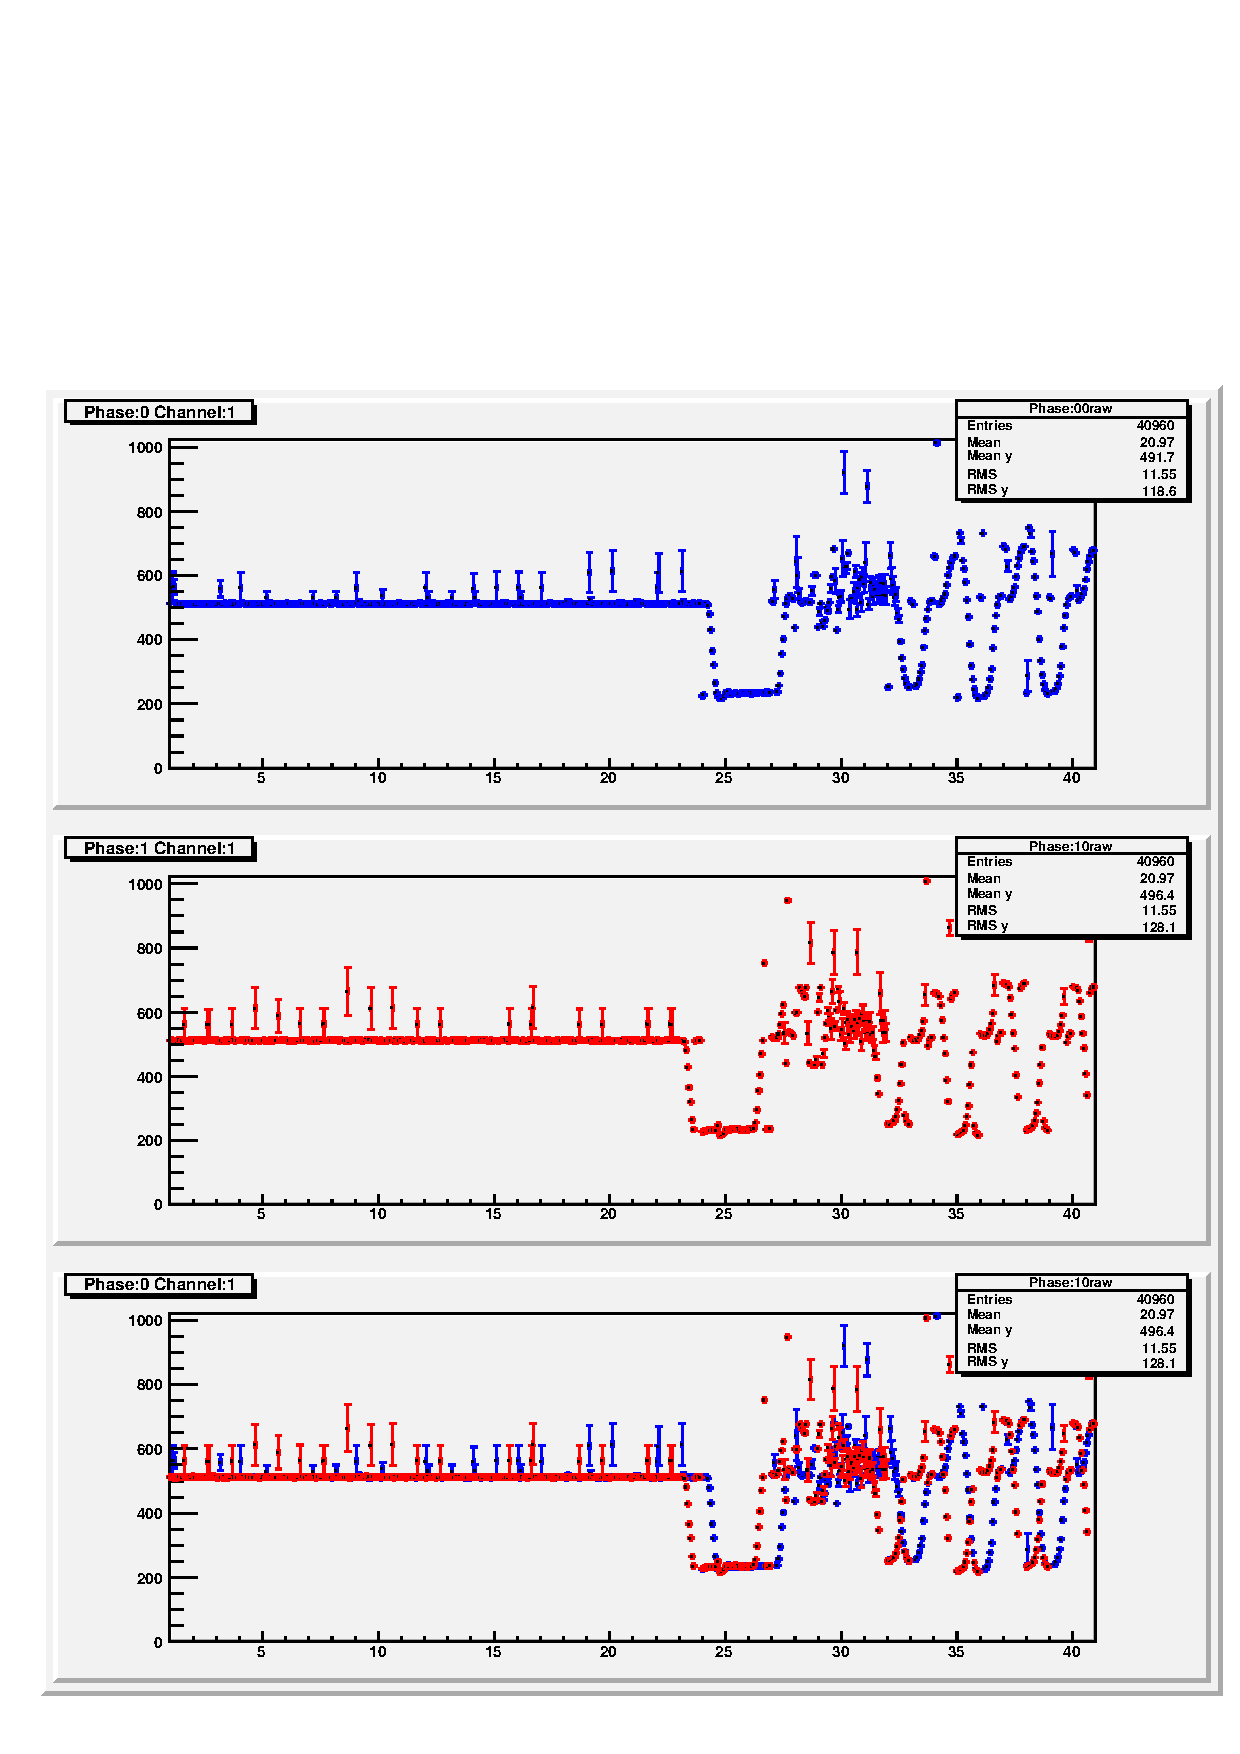
\includegraphics[width=\linewidth]{phaseAndDelayPlotRaw_channe_1_1}
\end{center}
\caption{This figure shows on top the adc value as a function of clock+delay/16 for phase=0 and the same plot for phase=1 in the middle. The two plots are overlaid at the bottom.}
\label{fig:phasedelayraw}
\end{figure}

We see that there are certain values of the delays that produce garbage as you try to read out the ADC before the data is available. To identify the invalid combinations of phase and delay I calculate the rms for the different phase and delay settings in the first 20 clock cycles, i.e. before the TBM header arrives. Based on the rms distribution it is seen that for phase=0 that we got invalid data with delays of 1, 2, and 3, while for phase=1 the delays of 10, 11, and 12 generate invalid data. From now on I will reject these combinations. (In the plots I set the adc value to 0.)

After rejecting the invalid phase and delay combinations we now have a signal that looks as what is shown in Fig.~\ref{fig:phasedelayvalid}.

\begin{figure}
\begin{center}
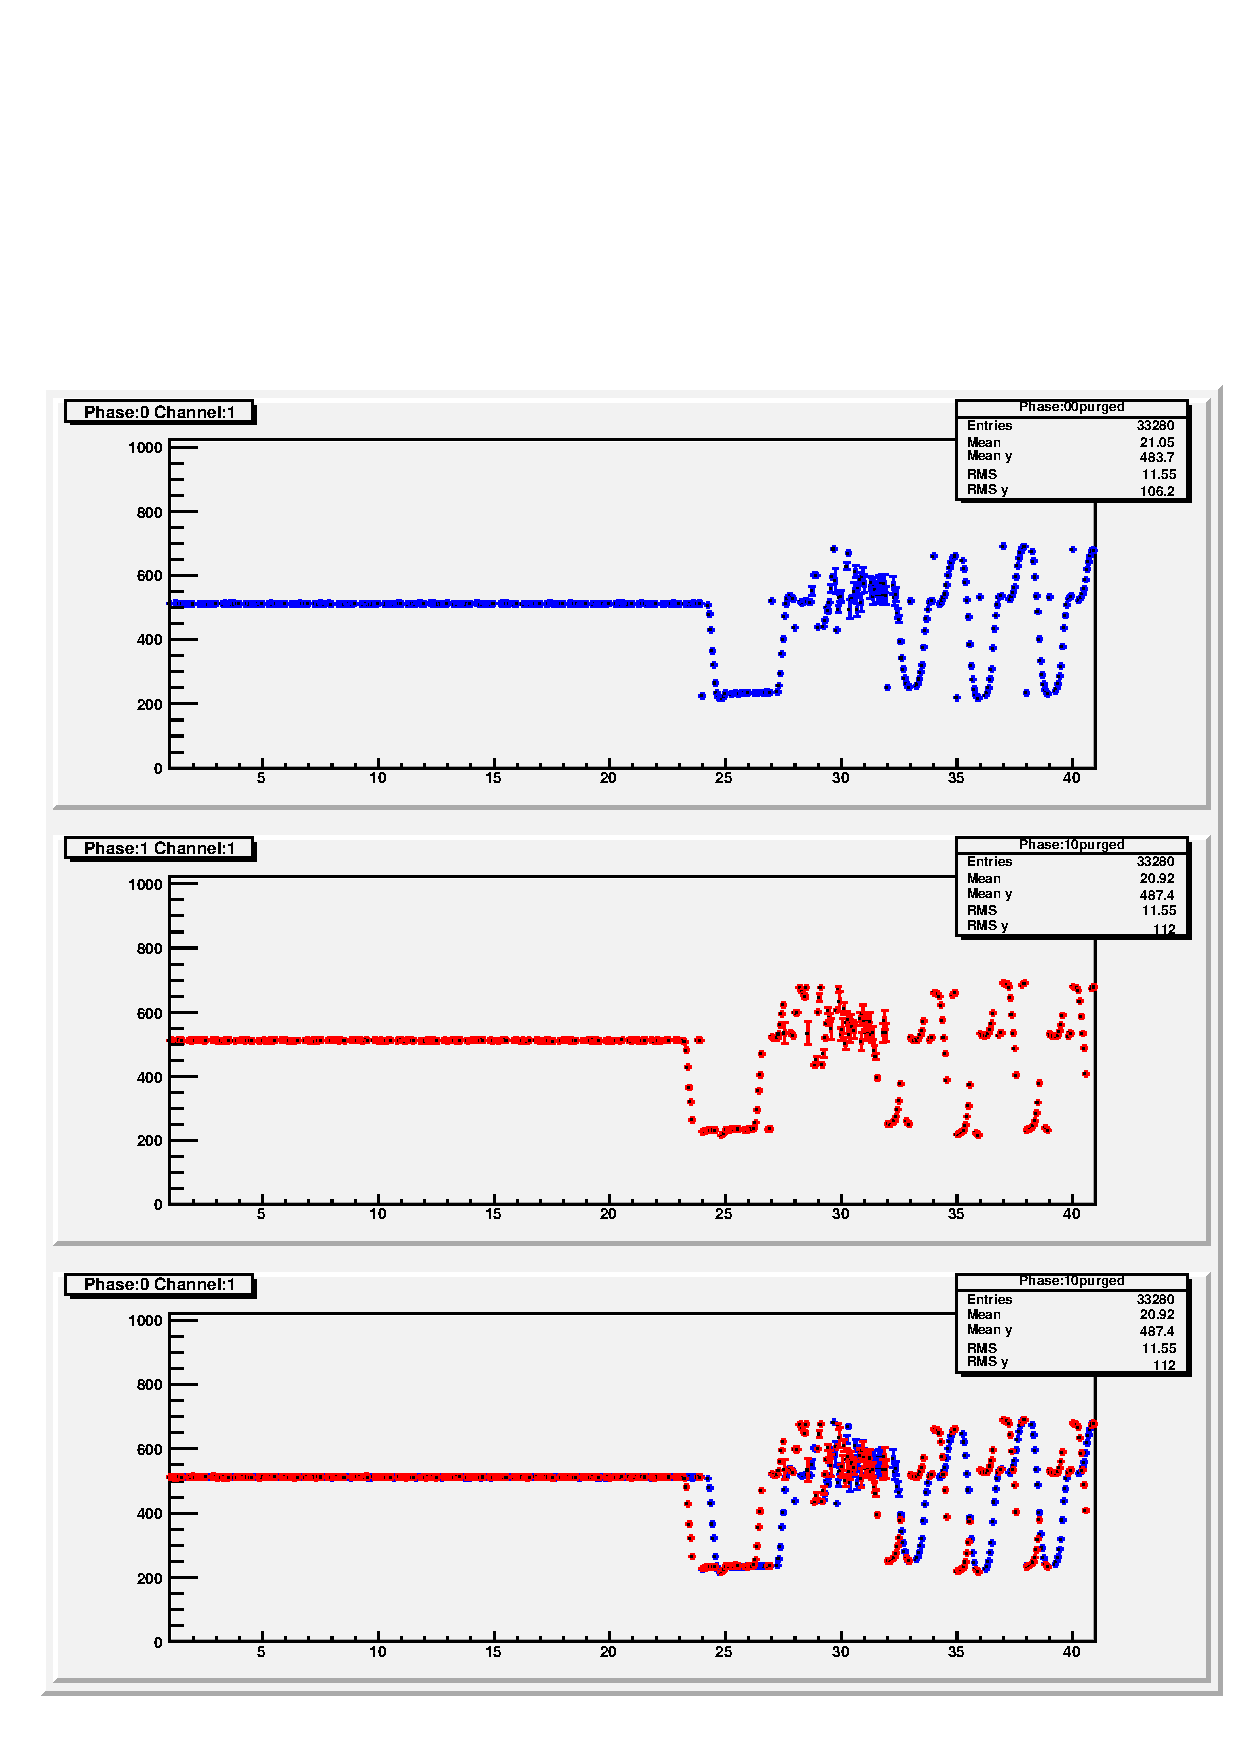
\includegraphics[width=\linewidth]{phaseAndDelayPlotPurged_channe_1_1}
\end{center}
\caption{This figure shows on top the adc value as a function of clock+delay/16 for phase=0 and the same plot for phase=1 in the middle. The two plots are overlaid at the bottom. Here I have set the adc value to 0 for the combinations of clock and phase that are not valid.}
\label{fig:phasedelayvalid}
\end{figure}

The remaining signal still has artifacts due to when the adc latches on to the signal such that it looks like the signal is not read out in order. This is corrected by 'reordering' the data within a clock. I shifted the phase=0 events backward by 3 delay steps and the phase 1 events forward by 3 delay steps. This makes the signal continuous as shown in Fig.~\ref{fig:phasedelayshifted}.

\begin{figure}
\begin{center}
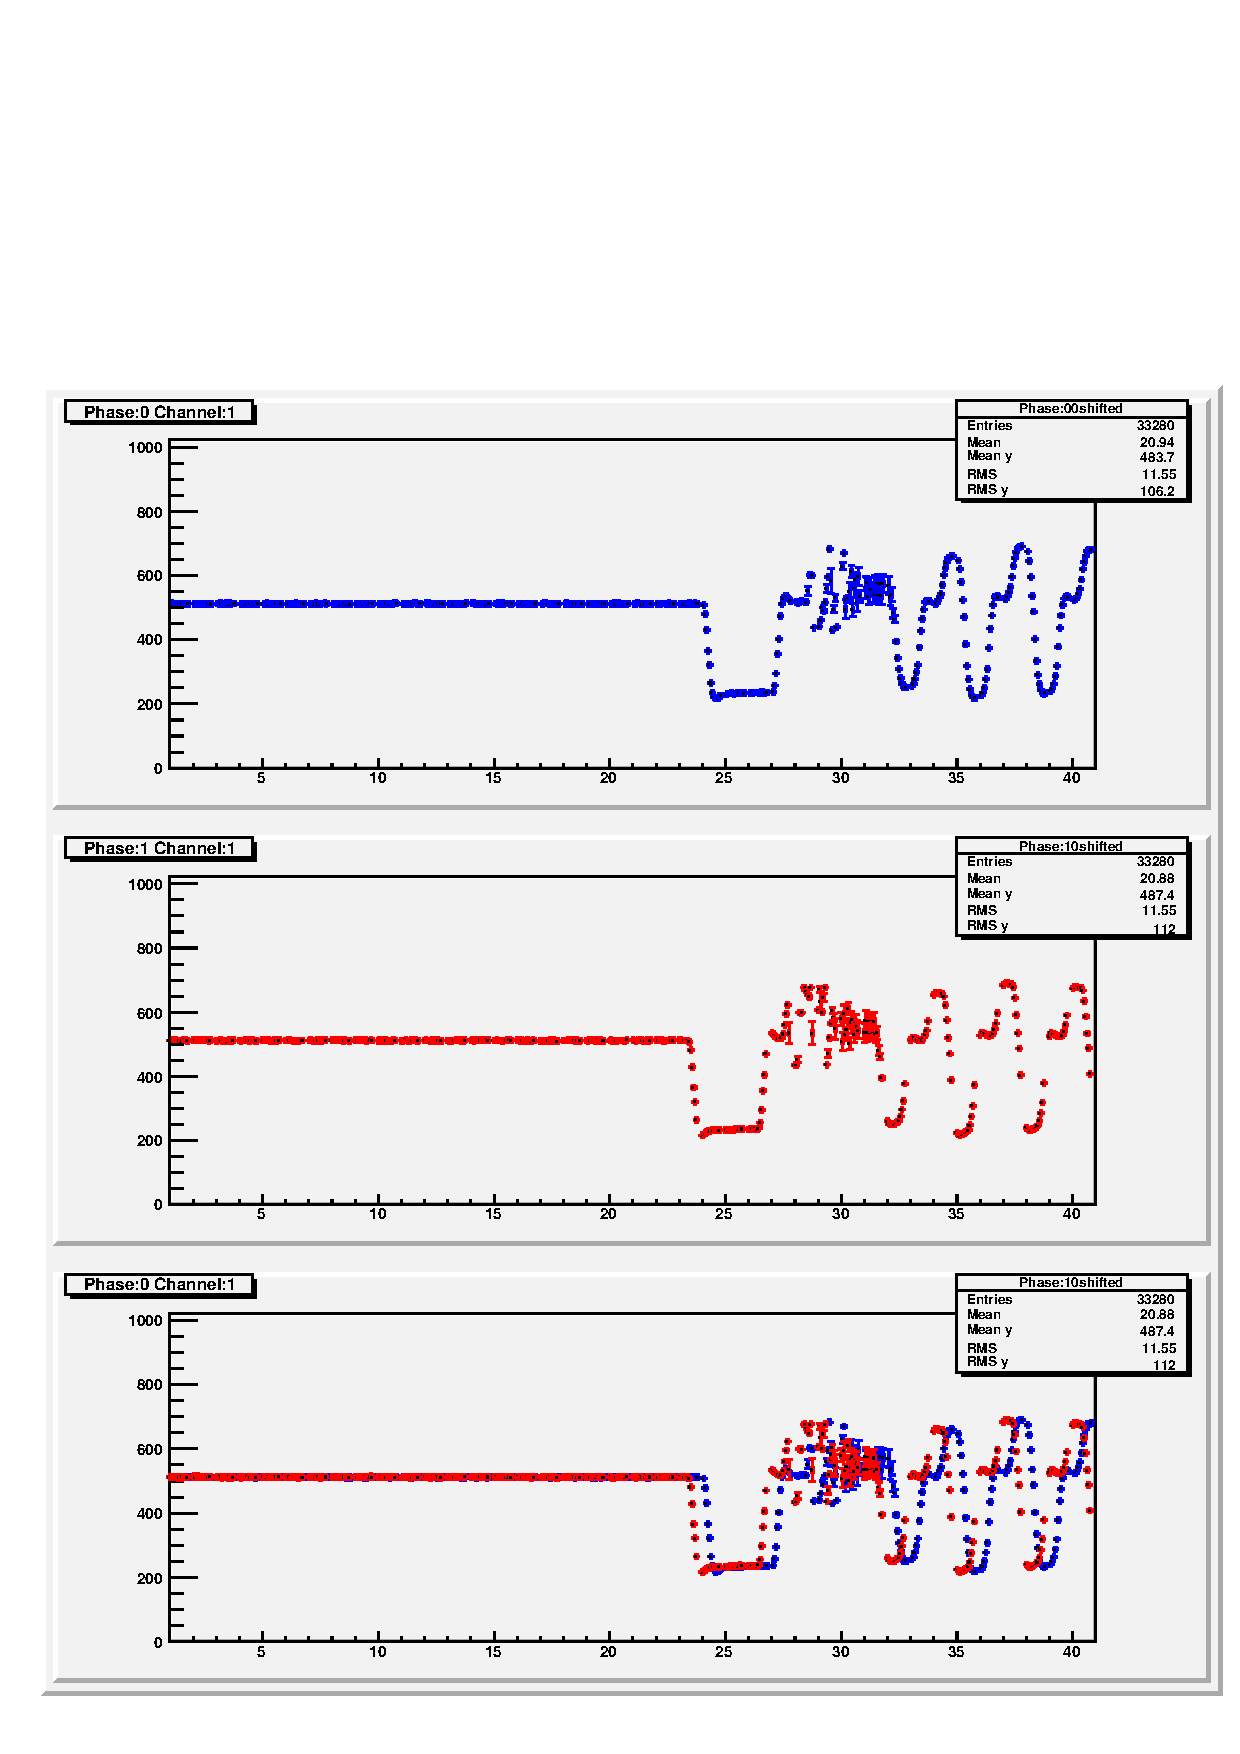
\includegraphics[width=\linewidth]{phaseAndDelayPlotShifted_channe_1_1}
\end{center}
\caption{This figure shows on top the adc value as a function of clock+delay/16 for phase=0 and the same plot for phase=1 in the middle. The two plots are overlaid at the bottom. Here the data within a clock has been ordered to give a continuous data signal.}
\label{fig:phasedelayshifted}
\end{figure}

The last step is to align the data so that the phase=0 and phase=1  data overlaps. I do this by shifting the data for the events with phase=1 by 10 delay steps. The final result is shown in  Fig.~\ref{fig:phasedelayfinal}. For the bins in the plot where there is data from both phase=0 and phase=1 we see that there is excellent agreement. We also note that the signal undershoots in a transition from black to ultrablack and that it overshoots on the reverse transition.

\begin{figure}
\begin{center}
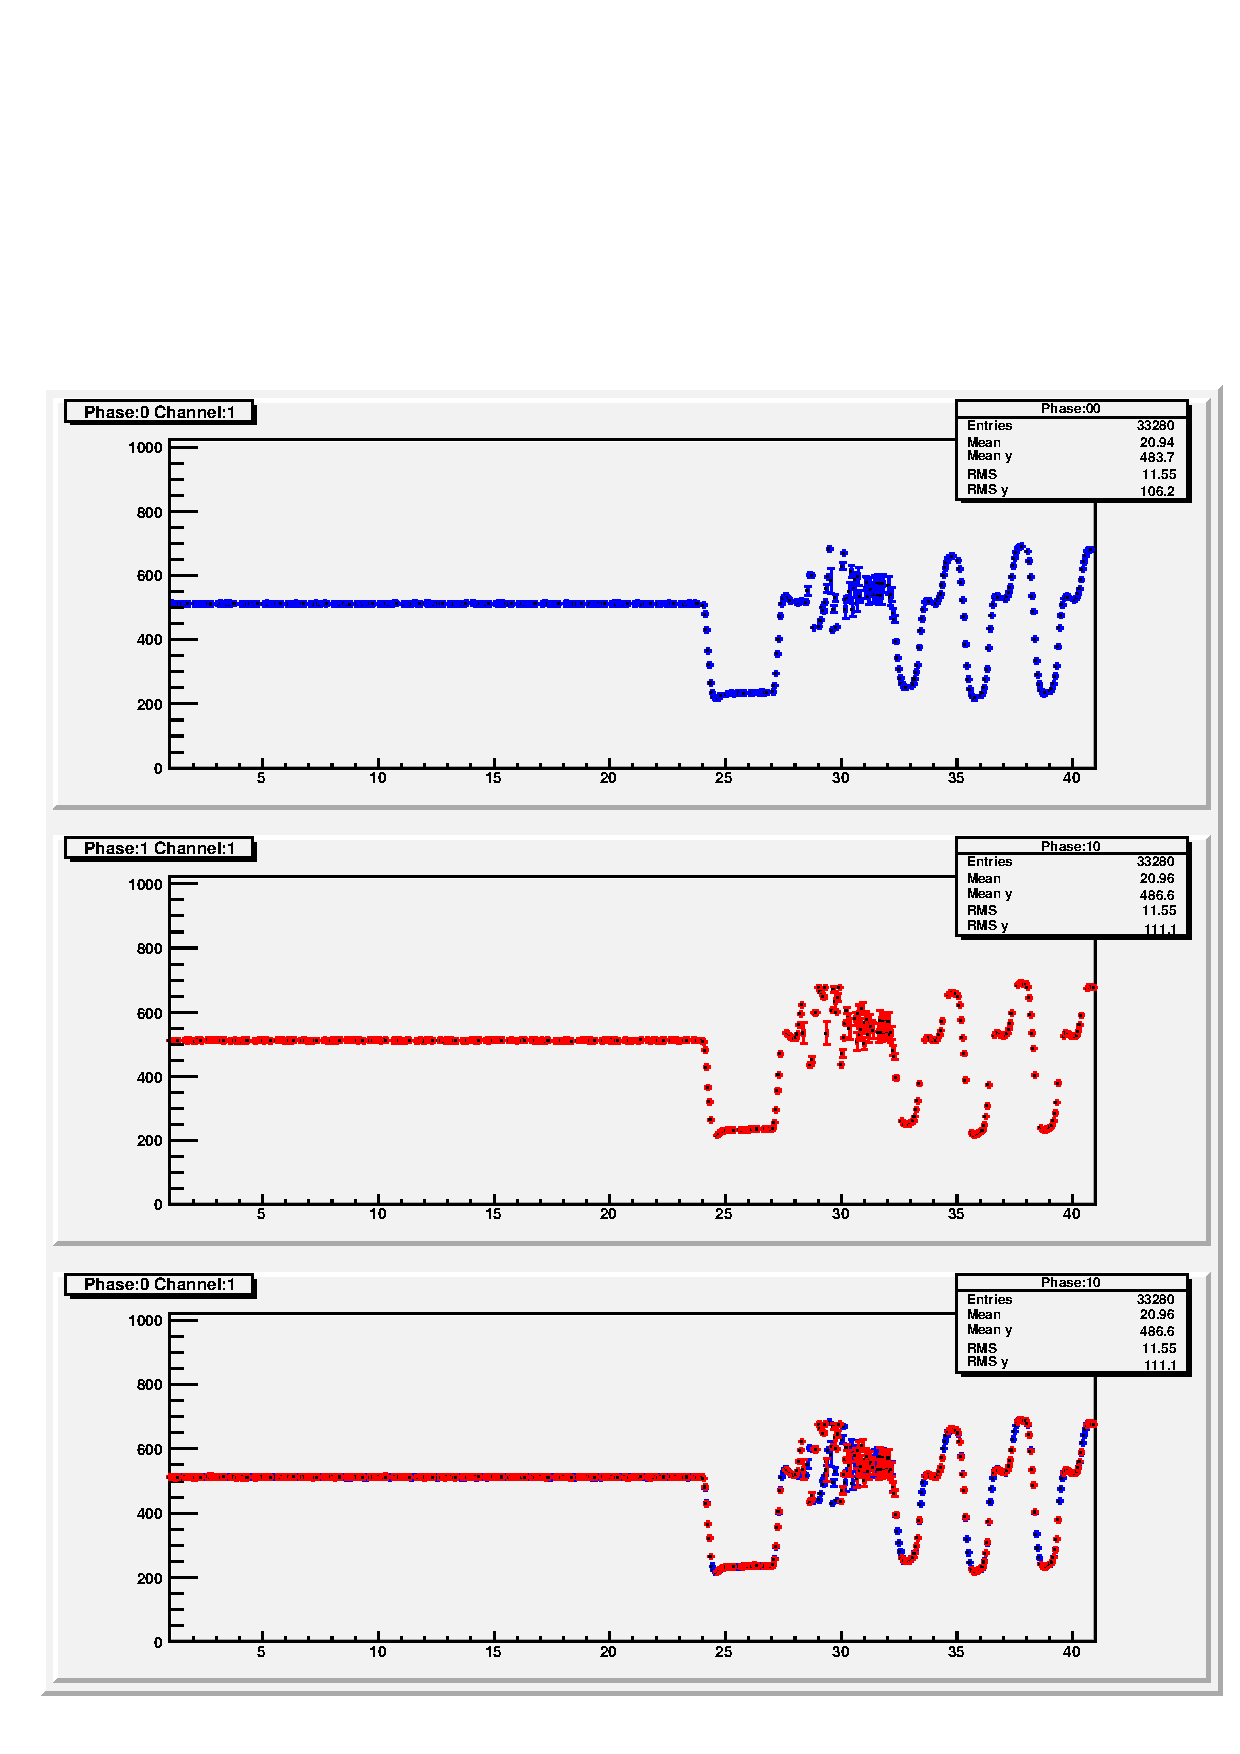
\includegraphics[width=\linewidth]{phaseAndDelayPlot_channe_1_1}
\end{center}
\caption{This figure shows on top the adc value as a function of clock+delay/16 for phase=0 and the same plot for phase=1 in the middle. The two plots are overlaid at the bottom. Here the phase=1 data has been shifted so that it overlaps with the phase=0 data.}
\label{fig:phasedelayfinal}
\end{figure}

To determine a best delay I look at the combined data - where I average the bins that has both phase=0 and phase=1 contributions - and calculate a difference for bin $i$ by taking the difference between bin $i-1$  and $i+1$. I calculate this difference for the 25 MHz clock cycles from clock 27 to 100. I add the magnitude of these differences for all bins that corresponds to the same delay. I pick the smallest such sum of differences for the different delay as the optimal choice. If more than one phase is allowed I pick the choice that is farthest from the invalid delay for that phase.

A new alogorithm has been implmented that determines the phase to be right at the edge of the transition from black to ultrablack in the TBM trailer. You can still run the old algorithm by setting the parameter 'oldMode' to 'Yes'.

Looking at the 8 channels that were connected to the pilot run detector I find that the results are very consistent. The phase is either 0 or 15 in the (aligned delay) for the raw delay setting this corresponds to 2 or 3 for phase=1.

Open questions: Is the same set of phases and delays illegal on all FEDs and channels? Also, are the shifts that are needed to time-order the data the same on all FEDs and channels? Looking at more data will resolve this. It is easy to test that the data in the two phases are compatible by forming a $\chi^2$.

The code was written as a root macro. I will 'transplant' this code into xdaq so we can run it automatically to produce the phase and delay settings needed.

However, looking at this I observed an odd feature. This is illustrated in Fig.~\ref{fig:phasedelaylatedata}.

\begin{figure}
\begin{center}
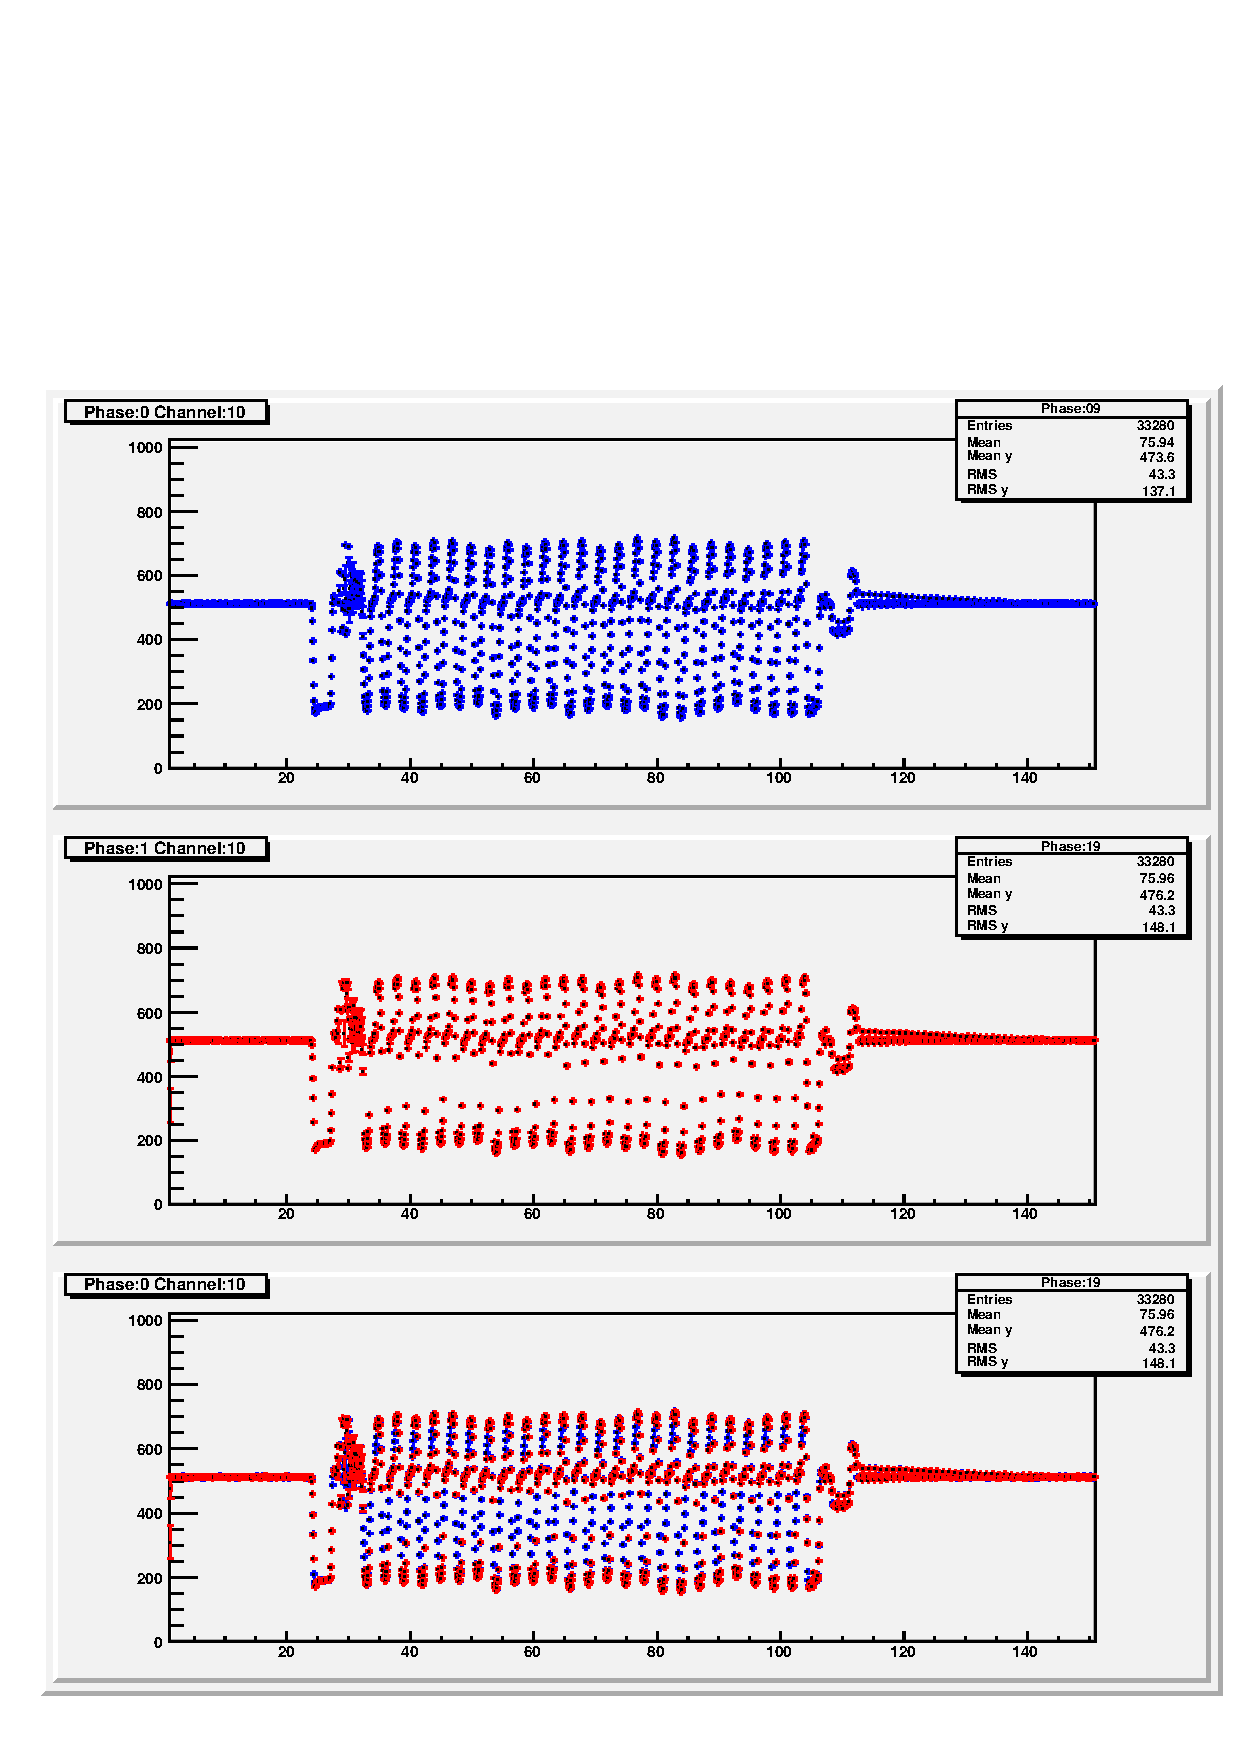
\includegraphics[width=\linewidth]{phaseAndDelayPlot_channe_10_1_latedata}
\end{center}
\caption{Here you see that for clocks in and after the TBM trailer that there is a feature in that some delays are oscillating. This 'excitation' seems to decay of after $O(20)$ clocks. }
\label{fig:phasedelaylatedata}
\end{figure}

In Fig.~\ref{fig:phasedelaylatedatazoom} is a close up of the region with the noise.

\begin{figure}
\begin{center}
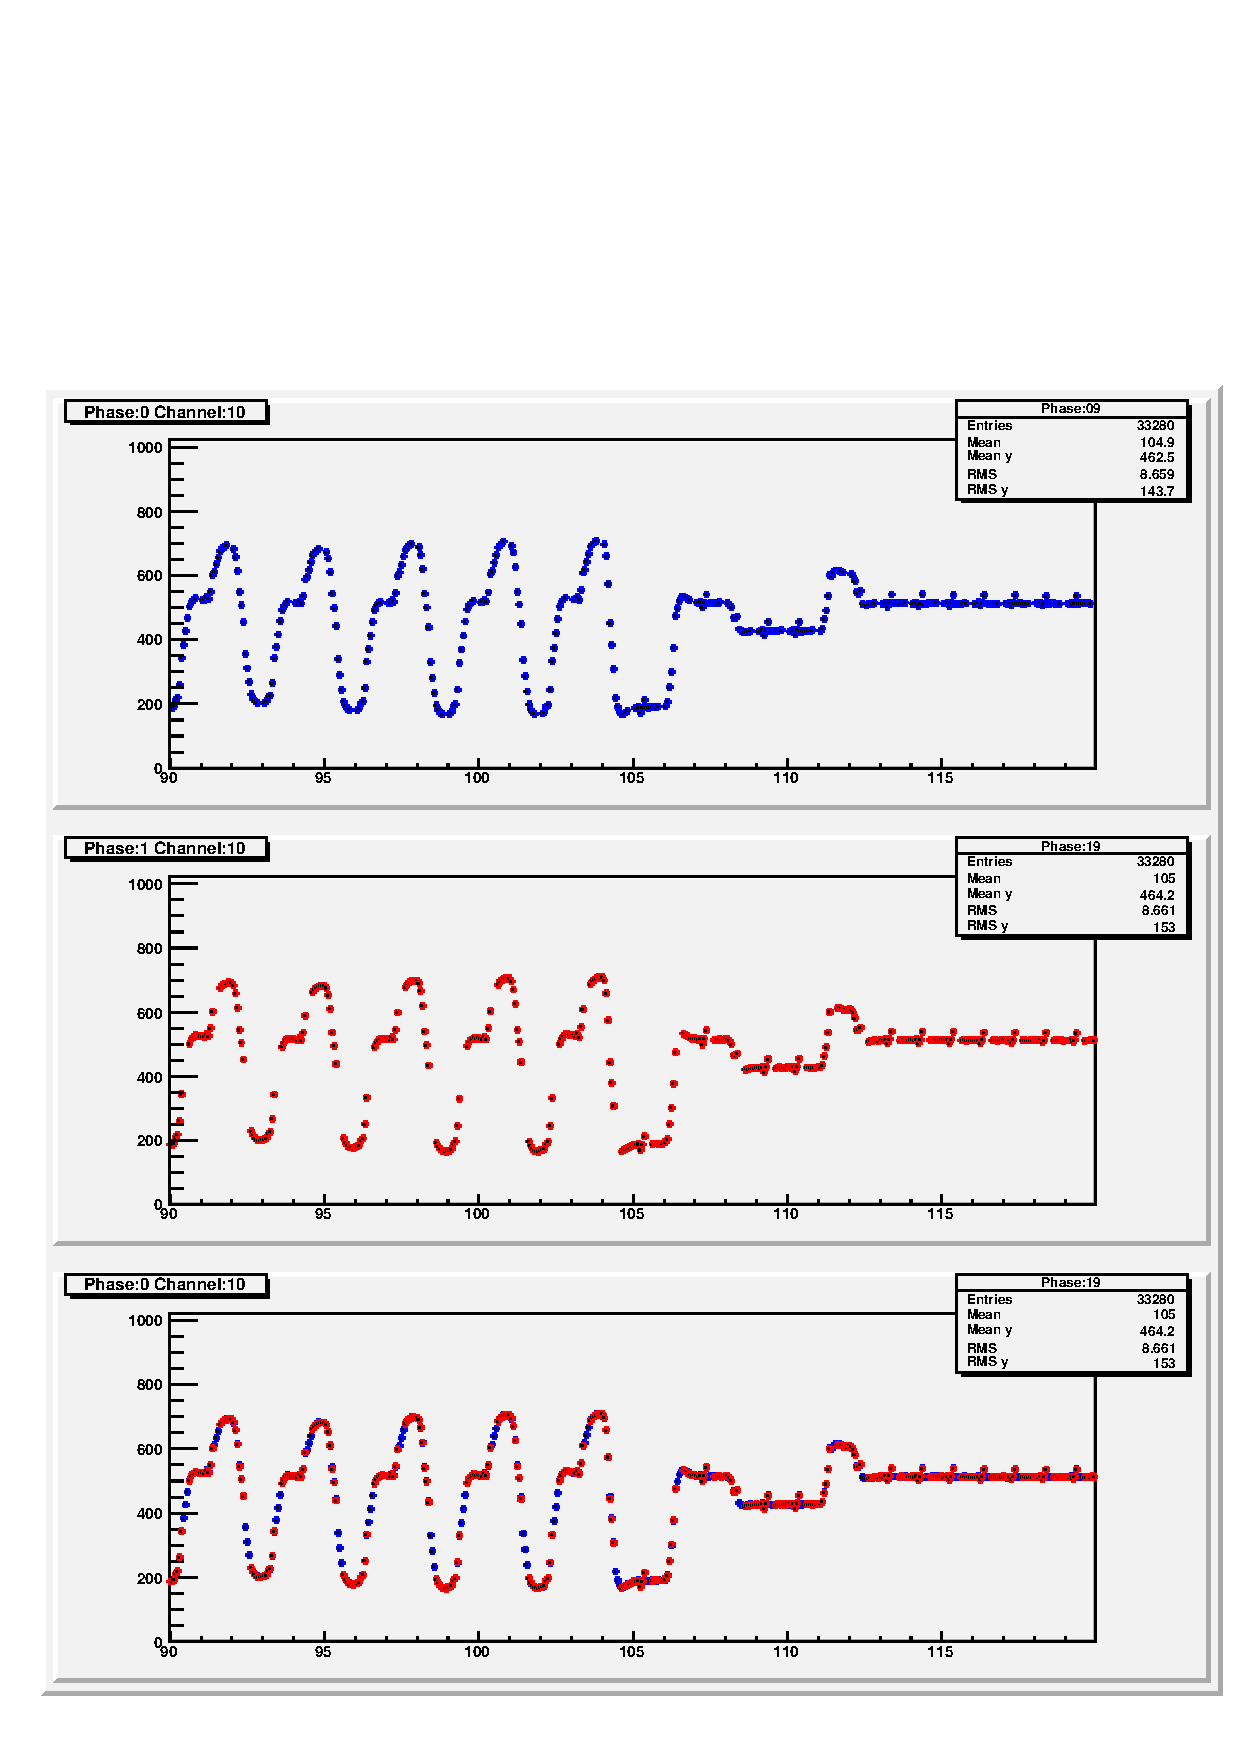
\includegraphics[width=\linewidth]{phaseAndDelayPlot_channe_10_1_latedatazoom}
\end{center}
\caption{Zooming in you can see that data in the two phases both agree on the shape of this feature. }
\label{fig:phasedelaylatedatazoom}
\end{figure}

Here you can see that there is 'wiggle' in the data that is large compared to the rms, as indicated by the error. This wiggle seems to persist for many clock cycles after the TBM trailer. However, it was not present in the black data before the data train. It seems to first start in the TBM trailer when the UB signal is generated. With the pilot run detector we are using 8 channels  (1, 2, 3, 4, 7, 8, 9, and 10). I see the same feature on  almost all channels, though they are not as strong on channel 1, 7, and 9. 

\begin{figure}
\begin{center}
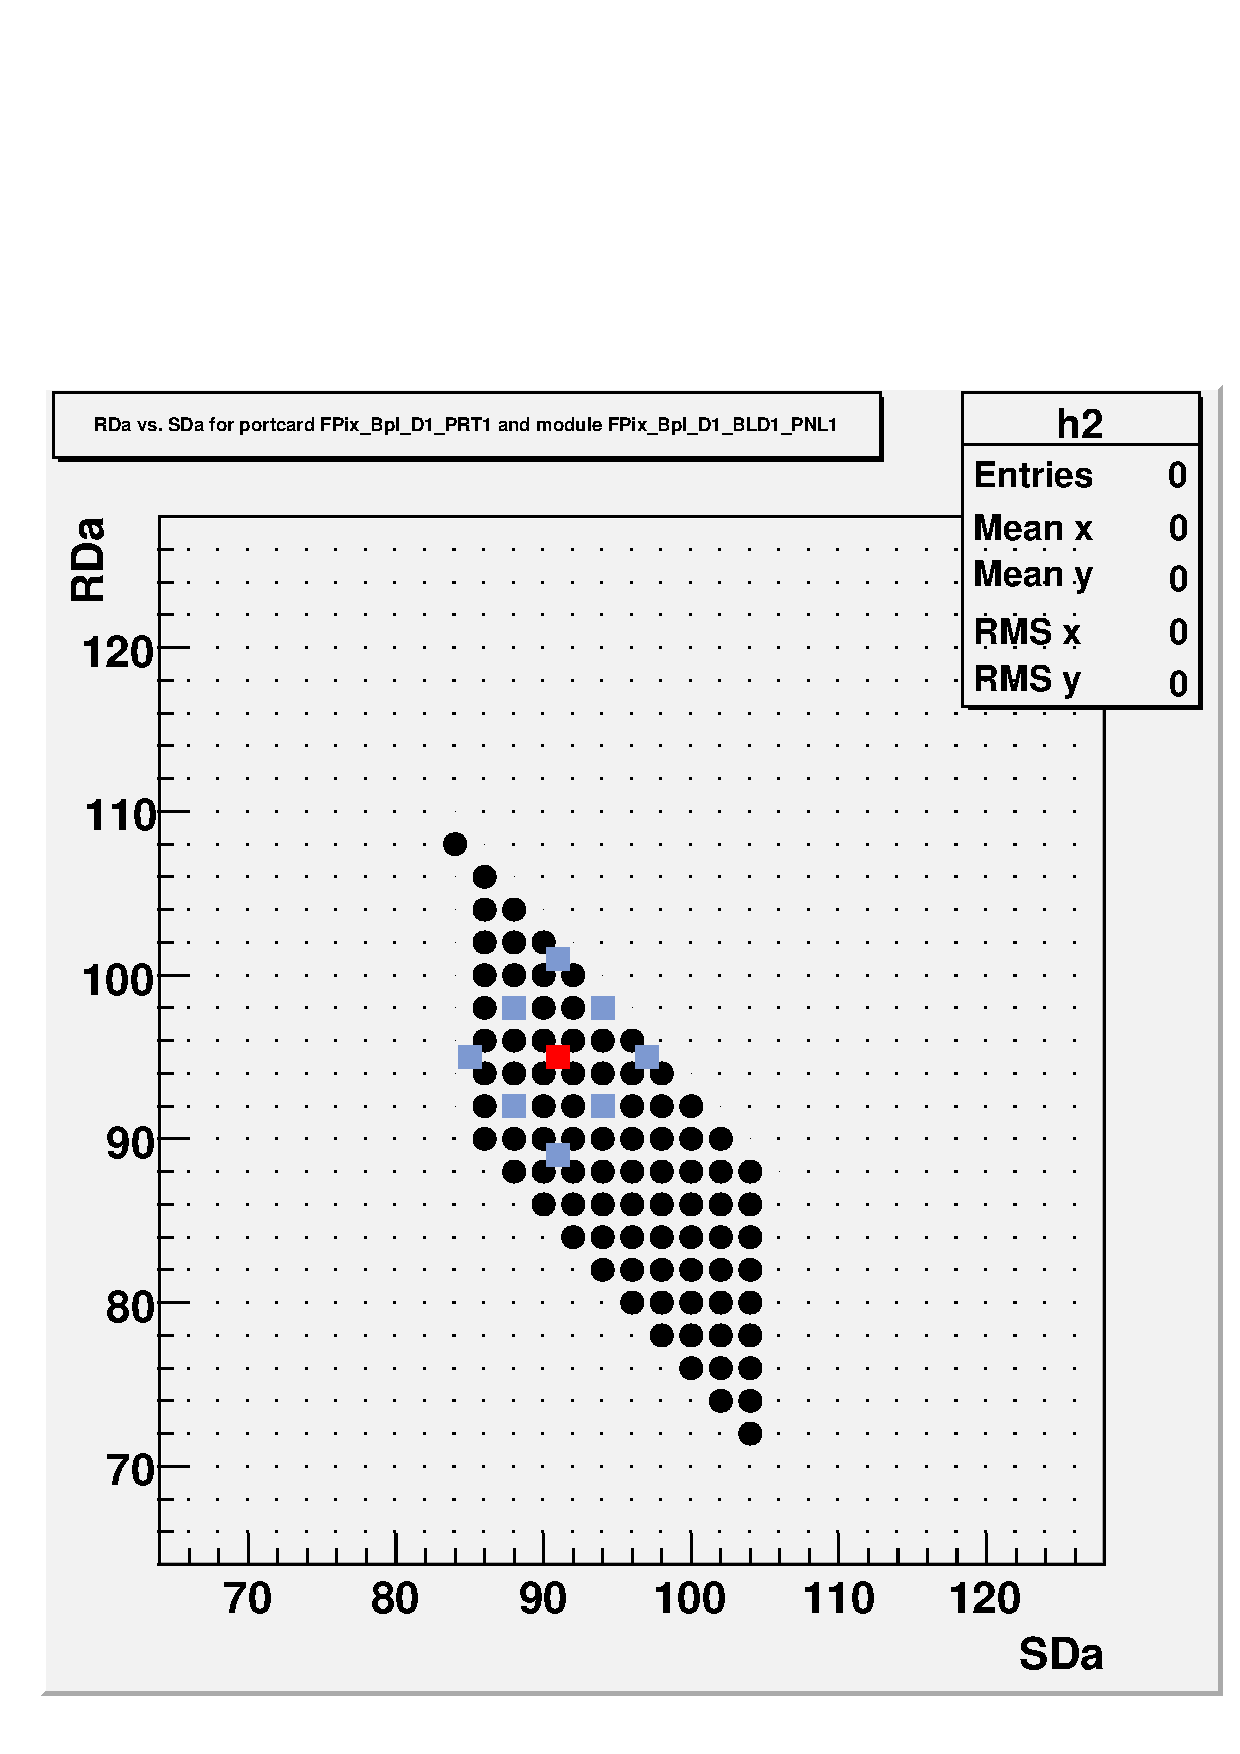
\includegraphics[width=0.48\linewidth]{graph_FPix_BpI_D1_PRT1_FPix_BpI_D1_BLD1_PNL1_0}
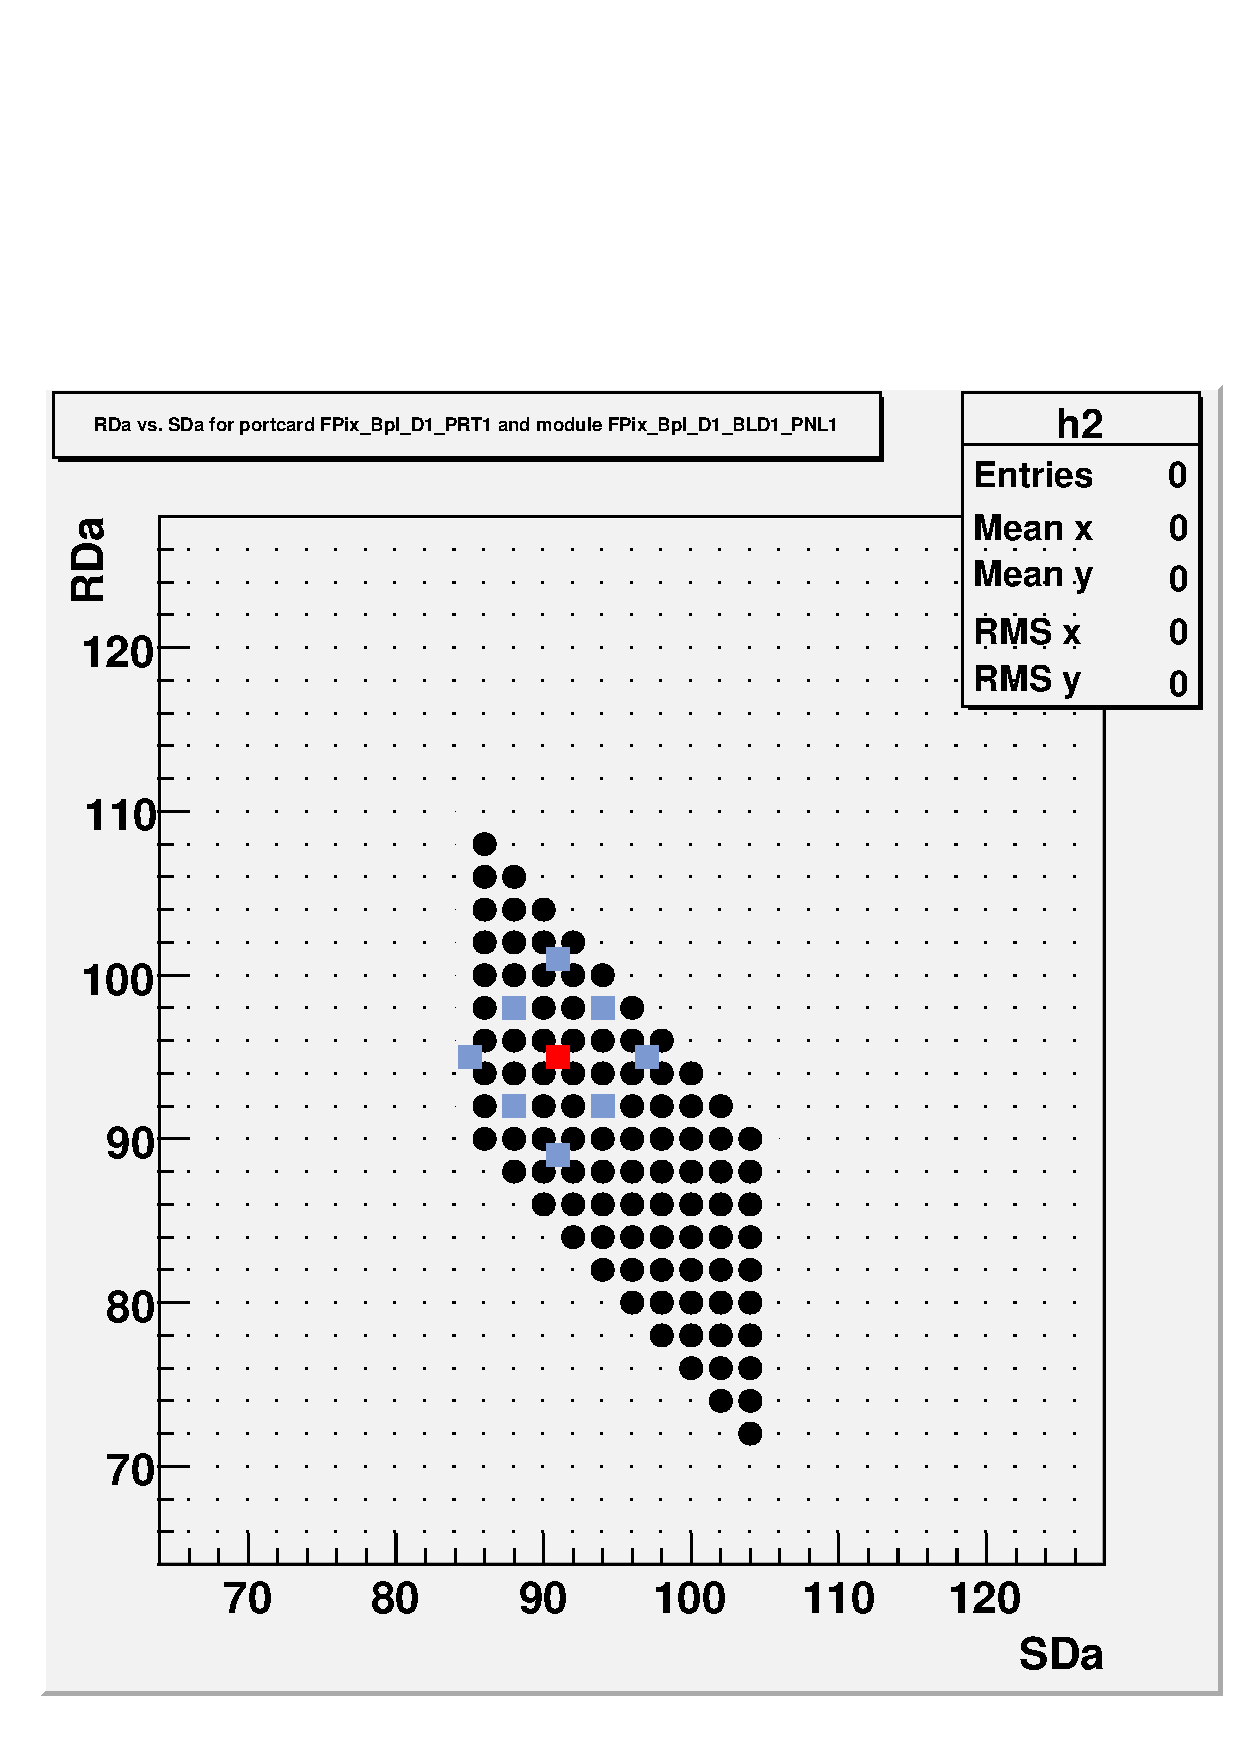
\includegraphics[width=0.48\linewidth]{graph_FPix_BpI_D1_PRT1_FPix_BpI_D1_BLD1_PNL1_1}
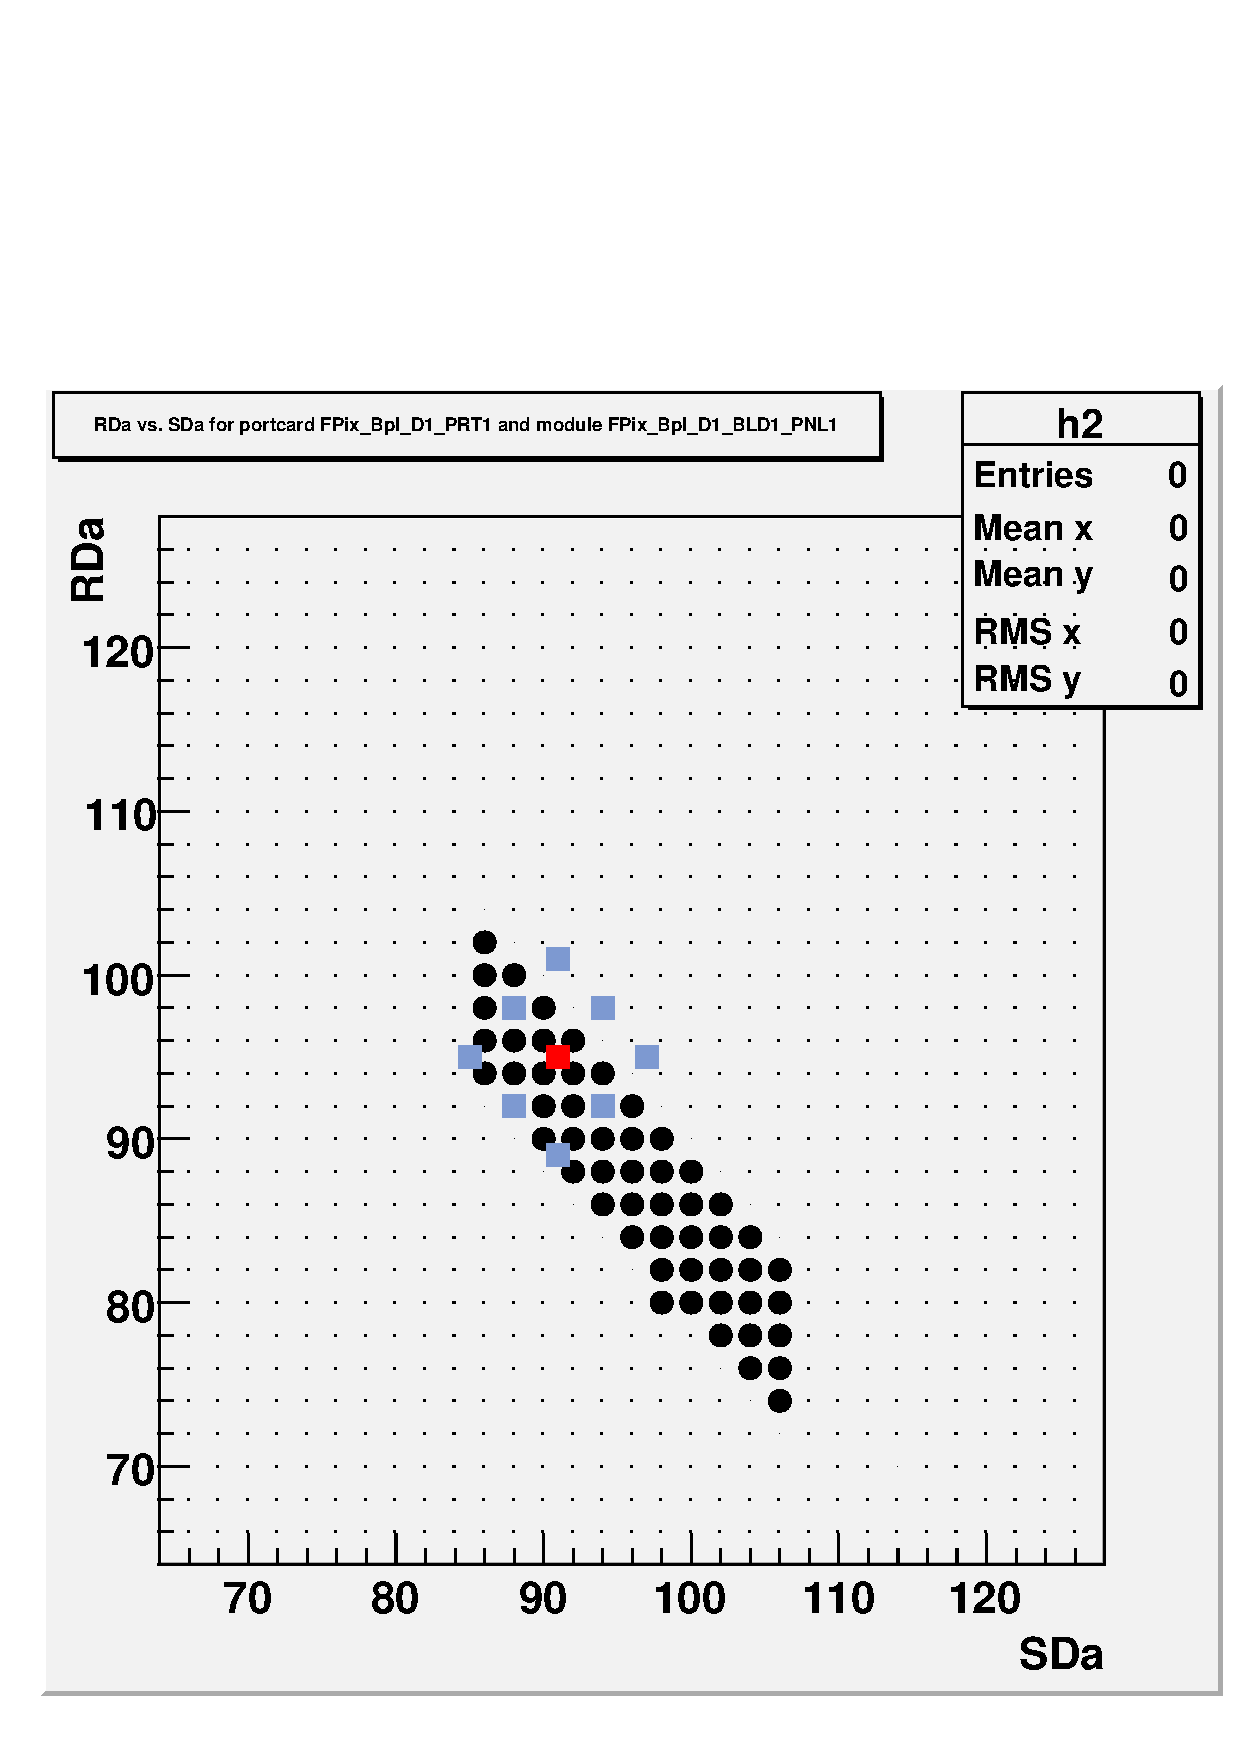
\includegraphics[width=0.48\linewidth]{graph_FPix_BpI_D1_PRT1_FPix_BpI_D1_BLD1_PNL1_2}
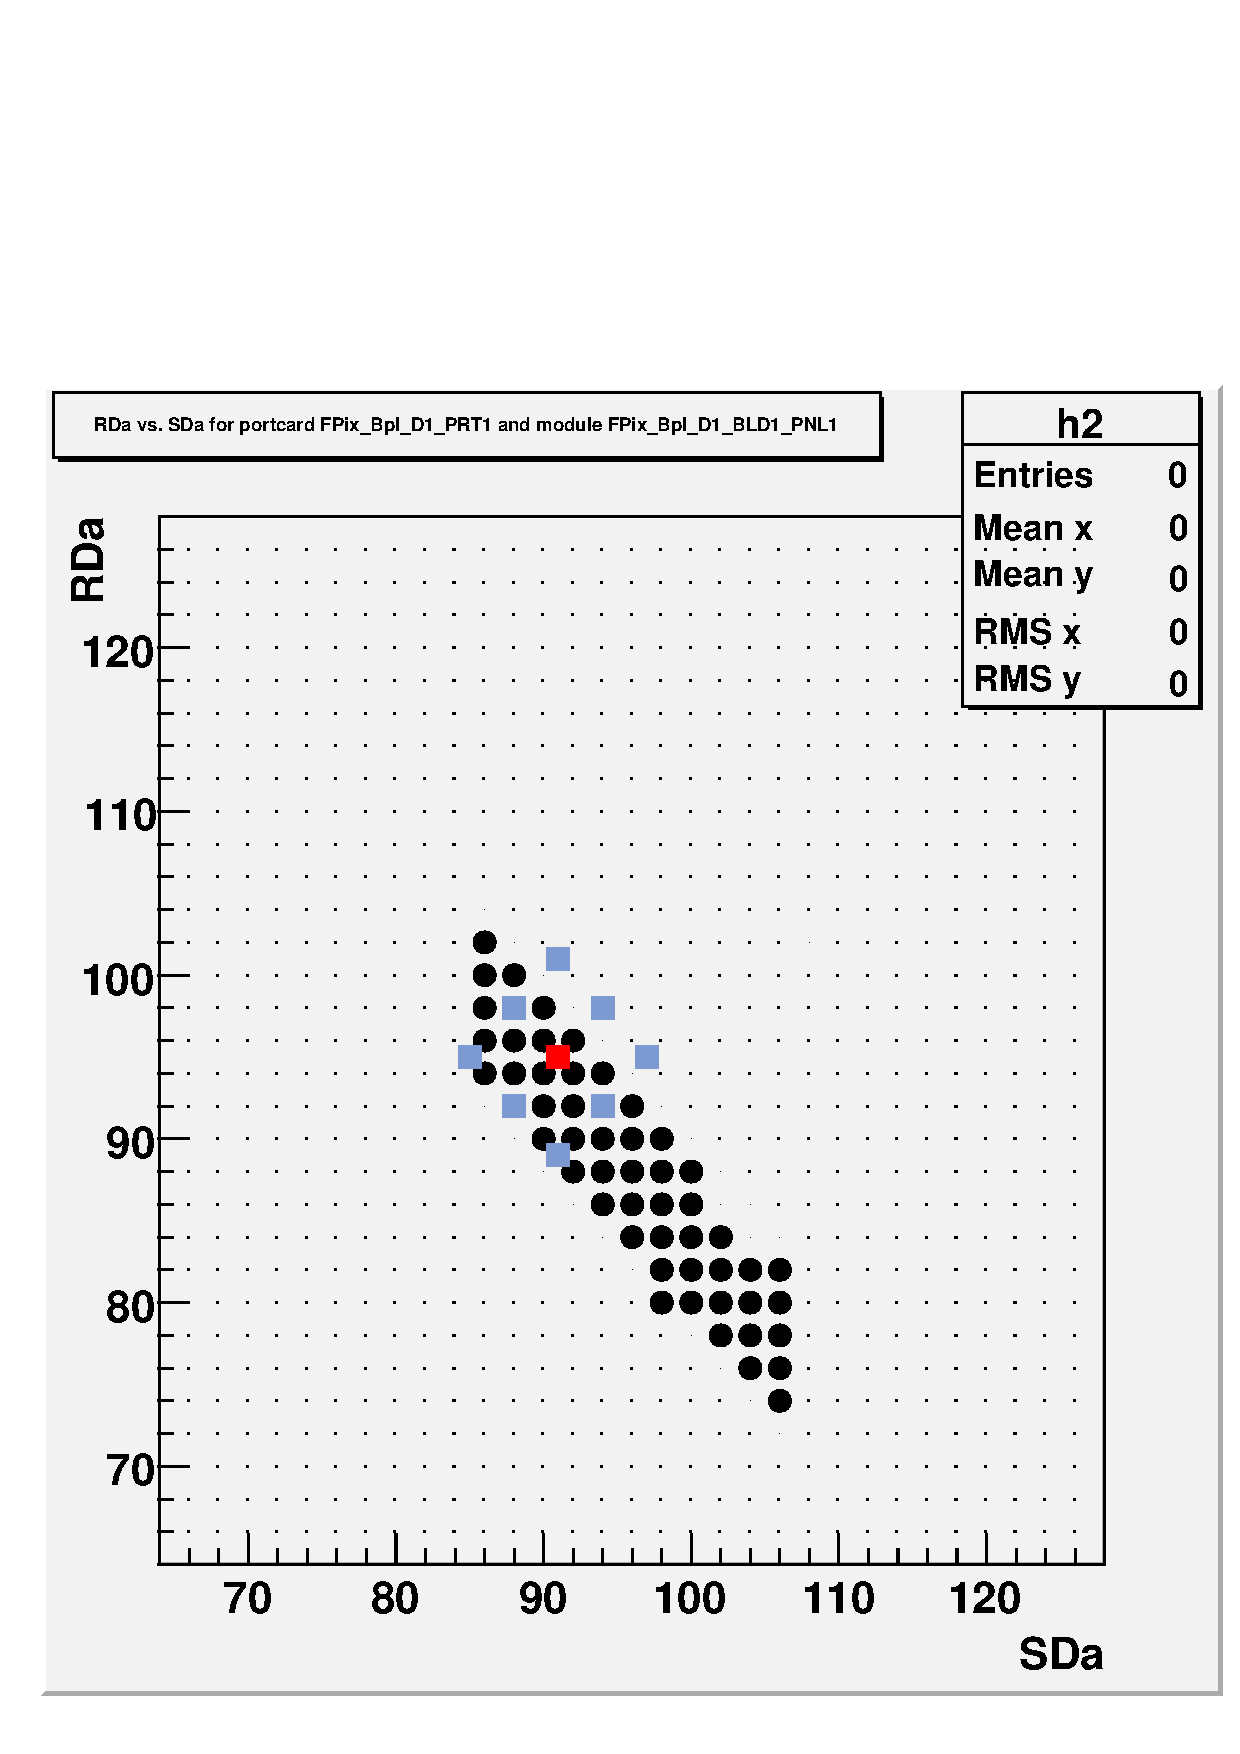
\includegraphics[width=0.48\linewidth]{graph_FPix_BpI_D1_PRT1_FPix_BpI_D1_BLD1_PNL1_3}
\end{center}
\caption{This figure shows the results of scans for delay25 settings on the Cornell test stand. The upper left plots shows (large black dots) the region for which the return data was valid when sending a ROC command (CalPix). The upper right plot shows the valid region when sending a TBM command (tbm speed). The lower left shows the region of success when sending a roc init and the lower right shows the region of success with a roc trim load command. As is seen, the working region is smaller for the long commands. The red and blue points indicates the algorithm used to select the operating point. Need to check with Jennifer what this is doing.}
\label{fig:scanDelay25}
\end{figure}

